% Esta puede ser la de datos 'random', si no creamos un otro archivo

\section{Misceláneo}

Se hará uso de la siguiente notación:
	\begin{itemize}
	    \item $k_B$ o $K_B$: constante de Boltzmann
	    \item \textit{N}: cantidad de moléculas en un sistema a estudiar
	    \item \textit{p}: presión
	    \item \textit{V}: volumen
	    \item \textit{E}: energía interna de un sistema
	    \item \textit{S}: entropía
	    \item $S_B$: entropía de un baño térmico
	    \item \textit{T}: temperatura (medida en Kelvin) (siempre $ T \geq 0$)
	    \item \textit{C}: capacidad calórica
	    \item $C_V$: capacidad calórica a volumen constante
	    \item $C_p$: capacidad calórica a presión constante
	    \item \textit{c}: calor específico
	    \item \textit{Q}: calor entregado \textit{al} sistema
	    
	    En caso de dos baños térmicos se tiene usualmente que:
	    \begin{itemize}
	        \item $Q_1$ es el baño \enquote{frío} 
	        \item $Q_2$ es el baño \enquote{caliente}
	    \end{itemize}
	    Ambos tienen temperaturas mayor a cero, pero $T_1 < T_2$
	    
	    \item \textit{W}: trabajo hecho \textit{sobre} el sistema
	\end{itemize}

\subsection{Fórmula de Stirling}

\[\ln n! \approx n\ln ( n )- n\]

\subsection{Mucha presión}

Si se ejerce una presión sobre un sistema mucho mayor a su presión interna, el sistema está fuera de equilibrio y por tanto no existe una única temperatura que lo caracterice.

\subsection{\textit{E(S,N,V)}}
\label{eq:e(s,v,n)}
Como al inicio del curso se tiene que $N$ es constante, entonces esto equivale a $E(S,V)$. Donde se obtiene $E$ a partir de la ecuación de Sackur-Tetrode y es para gases ideales monoatómicos.

\[ E(S,N,V) = \frac{3N}{4 \pi m}\lados{(}{\frac{Nh^3}{V}}^{(2/3)}\exp\lados{[}{\frac{2S}{3Nk_B} - \frac{5}{3}} \]

\subsection{Ciclo de Carnot en imágenes}
A la izquierda corresponde a un diagrama \textit{p-V} y el de la derecha a uno \textit{S-T}.

\begin{figure}[H]
    \centering
    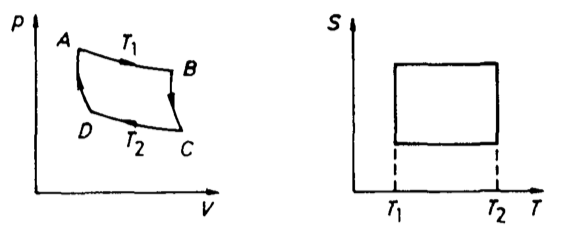
\includegraphics[width=0.65\textwidth]{img/ciclo_carnot.png}
    \caption{Diagrama ciclo de Carnot}
    \label{fig:diag_carnot}
\end{figure}

\subsection{Diferencial de Entalpía}

\[dH = C_pdT - \lados{[}{T\devtermo{p}{V}{T} - V}dp\]

\subsection{Relación cíclica}
\label{sub:relacion_ciclica}
Sea $z = z(x, y) \in \mathcal{C}^n$, con $n \geq 2$ entonces se tiene que:

\[\devtermo{y}{z}{x}\devtermo{z}{x}{y}\devtermo{x}{y}{z} = -1\]

\subsection{Coeficientes de expansión}

\begin{itemize}
    \item Coeficiente de expansión isotérmica
    \[ \beta \equiv -\devtermo{T}{V}{p}\frac{1}{V} \]
    
    \item Coeficiente de expansión térmica
    \[ \alpha \equiv \devtermo{p}{V}{T}\frac{1}{V} \]
\end{itemize}

\begin{equation}
\begin{split}
    \implies C_p &= C_V - T\devtermo{p}{V}{T}\devtermo{V}{p}{T}\\
                 &= C_V + TV\frac{\alpha^2}{\beta} 
\end{split}
\nonumber
\end{equation}